% do not change these two lines (this is a hard requirement
% there is one exception: you might replace oneside by twoside in case you deliver 
% the printed version in the accordant format
\documentclass[11pt,titlepage,oneside,openany]{book}
\usepackage{times}

%personally added
\usepackage{color}

\usepackage{graphicx}
\usepackage{latexsym}
\usepackage{amsmath}
\usepackage{amssymb}


\usepackage{ntheorem}

% \usepackage{paralist}
\usepackage{tabularx}

% this packaes are useful for nice algorithms
\usepackage{algorithm}
\usepackage{algorithmic}

% well, when your work is concerned with definitions, proposition and so on, we suggest this
% feel free to add Corrolary, Theorem or whatever you need
\newtheorem{definition}{Definition}
\newtheorem{proposition}{Proposition}


% its always useful to have some shortcuts (some are specific for algorithms
% if you do not like your formating you can change it here (instead of scanning through the whole text)
\renewcommand{\algorithmiccomment}[1]{\ensuremath{\rhd} \textit{#1}}
\def\MYCALL#1#2{{\small\textsc{#1}}(\textup{#2})}
\def\MYSET#1{\scshape{#1}}
\def\MYAND{\textbf{ and }}
\def\MYOR{\textbf{ or }}
\def\MYNOT{\textbf{ not }}
\def\MYTHROW{\textbf{ throw }}
\def\MYBREAK{\textbf{break }}
\def\MYEXCEPT#1{\scshape{#1}}
\def\MYTO{\textbf{ to }}
\def\MYNIL{\textsc{Nil}}
\def\MYUNKNOWN{ unknown }
% simple stuff (not all of this is used in this examples thesis
\def\INT{{\mathcal I}} % interpretation
\def\ONT{{\mathcal O}} % ontology
\def\SEM{{\mathcal S}} % alignment semantic
\def\ALI{{\mathcal A}} % alignment
\def\USE{{\mathcal U}} % set of unsatisfiable entities
\def\CON{{\mathcal C}} % conflict set
\def\DIA{\Delta} % diagnosis
% mups and mips
\def\MUP{{\mathcal M}} % ontology
\def\MIP{{\mathcal M}} % ontology
% distributed and local entities
\newcommand{\cc}[2]{\mathit{#1}\hspace{-1pt} \# \hspace{-1pt} \mathit{#2}}
\newcommand{\cx}[1]{\mathit{#1}}
% complex stuff
\def\MER#1#2#3#4{#1 \cup_{#3}^{#2} #4} % merged ontology
\def\MUPALL#1#2#3#4#5{\textit{MUPS}_{#1}\left(#2, #3, #4, #5\right)} % the set of all mups for some concept
\def\MIPALL#1#2{\textit{MIPS}_{#1}\left(#2\right)} % the set of all mips


% custom stuff
\usepackage[hidelinks]{hyperref}


\begin{document}

\pagenumbering{roman}
% lets go for the title page, something like this should be okay
\begin{titlepage}
	\vspace*{2cm}
  \begin{center}
   {\huge Mining the Success for Movies \\}
   \vspace{2cm} 
   {\Large Student Project Data Mining HWS17\\
   Team 6\\}
   \vspace{2cm}
   {\Large Presented by \\}
   \vspace{0.5cm}
    {Steffen Jung \\
    Adrian Kochsiek \\
    Martin Koller \\
    Marvin Messenzehl \\
    Daniel Szymkowiak \\
   }
   \vspace{1cm} 
   { Submitted to the\\
    Data and Web Science Group\\
    Prof.\ Dr.\ Heiko Paulheim\\
    University of Mannheim\\} \vspace{2cm}
   {October - December 2017}
  \end{center}
\end{titlepage} 

% no lets make some add some table of contents
\tableofcontents
\newpage

\listofalgorithms

\listoffigures

\listoftables

% evntuelly you might add something like this
% \listtheorems{definition}
% \listtheorems{proposition}

\newpage


% okay, start new numbering ... here is where it really starts
\pagenumbering{arabic}

%%%%%%%%%%%%%%%%%%%%%%%%%%%%%%%%%%%%%%%%

% INPUTS
\chapter{Data Selection}

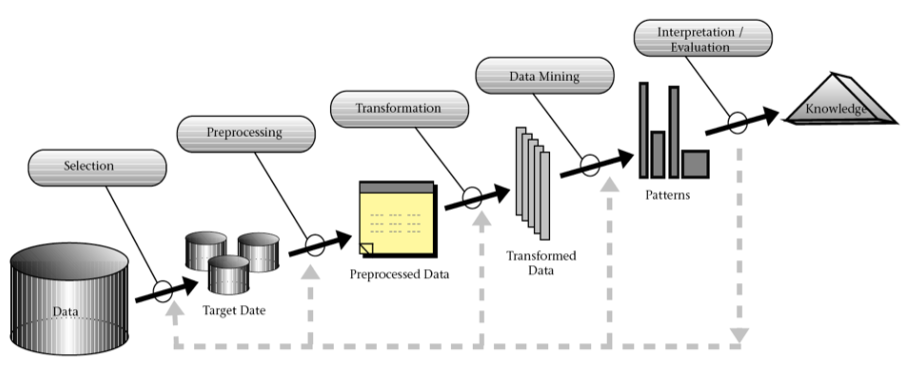
\includegraphics[width=\textwidth]{images/DM_Process.png}

\begin{itemize}
	\item Selection: 
	\begin{itemize}
		\item What data is available?
		\item What do I know about the provenance of the data?
		\item What do I know about the quality of the data?
	\end{itemize}
	\item Exploration
	\begin{itemize}
		\item Get an intitial understanding of the data
		\item Calculate basic summarization statistics
		\item Visualize the data
		\item Identify data problems such as outliers, missing values, duplicate records
	\end{itemize}
\end{itemize}

\chapter{Preprocessing and Transformation}
\begin{itemize}
\item Transform data into a representation that is suitable for the chosen data mining methods
\begin{itemize}
\item number of dimensions
\item scales of attributes (nominal, ordinal, numeric)
\item amount of data (determines hardware requirements)
\end{itemize}
\item Methods
\begin{itemize}
\item Aggregation, sampling
\item Dimensionality reduction / feature subset selection
\item Attribute transformation / text to term vector
\item Discretization and binarization
\end{itemize}
\item Good data preparation is key to producing valid and reliable models
\item Data preparation estimated to take 70-80\% of the time and effort of a data mining project!
\end{itemize}

\chapter{Data Mining}
\begin{itemize}
\item Input: Preprocessed Data
\item Output: Model / Patterns
\end{itemize}

\begin{enumerate}
\item Apply data mining method
\item Evaluate resulting model / patterns
\item Iterate:
\begin{itemize}
\item Experiment with different parameter settings
\item Experiment with different alternative methods – Improve preprocessing and feature generation – Combine different methods
\end{itemize}
\end{enumerate}

\chapter{Interpretation / Evaluation}
\begin{itemize}
	\item Output of Data Mining
	\begin{itemize}
		\item Patterns
		\item Models
	\end{itemize}
	\item In the end, we want to derive value from that, e.g.,
	\begin{itemize}
		\item gain knowledge
		\item make better decisions
		\item increase revenue
	\end{itemize}
\end{itemize}




%\input{./content/outline.tex}

\bibliographystyle{plain}
\bibliography{literature}




%not needed as stated in dws_vorlage
%\appendix

%\chapter{Program Code / Resources}
%\label{cha:appendix-a}

%The source code, a documentation, some usage examples, and additional test results are available at ...

%They as well as a PDF version of this thesis is also contained on the CD-ROM attached to this thesis.

%\chapter{Further Experimental Results}
%\label{cha:appendix-b}

%In the following further experimental results are ...




\newpage


\pagestyle{empty}


%\section*{Ehrenw\"ortliche Erkl\"arung}
%Ich versichere, dass ich die beiliegende Master-/Bachelorarbeit ohne Hilfe Dritter
%und ohne Benutzung anderer als der angegebenen Quellen und Hilfsmittel
%angefertigt und die den benutzten Quellen w\"ortlich oder inhaltlich
%entnommenen Stellen als solche kenntlich gemacht habe. Diese Arbeit
%hat in gleicher oder \"ahnlicher Form noch keiner Pr\"ufungsbeh\"orde
%vorgelegen. Ich bin mir bewusst, dass eine falsche Er- kl\"arung rechtliche Folgen haben
%wird.
%\\
%\\

%\noindent
%Mannheim, den 31.08.2014 \hspace{4cm} Unterschrift

\end{document}
